\documentclass[10pt,a4paper]{article}
\usepackage[T1]{fontenc}
\usepackage{lmodern}
\usepackage[margin=1.7cm]{geometry}
\usepackage{amsmath,amssymb}
\usepackage{booktabs,array,tabularx}
\usepackage{enumitem}
\usepackage[dvipsnames]{xcolor}
\usepackage{tikz}
\usetikzlibrary{arrows.meta,positioning}
\usepackage[most]{tcolorbox}
\usepackage{fancyhdr}
\usepackage[colorlinks=true,linkcolor=NavyBlue,urlcolor=NavyBlue]{hyperref}

\setlist{nosep,leftmargin=*}
\setlength{\parindent}{0pt}
\setlength{\parskip}{3pt}

\pagestyle{fancy}
\fancyhf{}
\lhead{\small BACSE202 -- Module 3}
\rhead{\small B-Tree \& B$^+$-Tree Indexing}
\cfoot{\thepage}

\newtcolorbox{keybox}[1][]{colback=NavyBlue!5,colframe=NavyBlue!70,fonttitle=\bfseries,title={#1},boxsep=2pt,left=4pt,right=4pt,top=2pt,bottom=2pt}
\newtcolorbox{exbox}[1][]{colback=ForestGreen!5,colframe=ForestGreen!70,fonttitle=\bfseries,title={#1},boxsep=2pt,left=4pt,right=4pt,top=2pt,bottom=2pt}
\newtcolorbox{warnbox}[1][]{colback=BrickRed!5,colframe=BrickRed!70,fonttitle=\bfseries,title={#1},boxsep=2pt,left=4pt,right=4pt,top=2pt,bottom=2pt}

% tree styles
\tikzset{
  bt/.style={>=Stealth, every node/.style={draw, rectangle, rounded corners=1pt, fill=NavyBlue!8, font=\small, inner sep=2.5pt, minimum height=5mm},
             edge from parent/.style={draw, -}, level distance=11mm},
  leaf/.style={fill=ForestGreen!12},
  link/.style={->, densely dashed, ForestGreen!70!black, shorten >=1pt, shorten <=1pt},
  tcap/.style={draw=none, fill=none, font=\scriptsize\itshape}
}
\newcommand{\sep}{\,$\mid$\,}

\begin{document}

\begin{center}
{\LARGE\bfseries BACSE202 -- Database Systems}\\[3pt]
{\Large B-Tree and B$^+$-Tree Indexing -- Complete Notes}\\[3pt]
{\small Module 3 (dynamic multilevel indexing). Built from the course slides (\texttt{BACSE202-DBS-Module-3}, slides 136--160; \texttt{Types\_of\_Indexes\_in\_DBMS}, slides 38--61) and Elmasri \& Navathe Ch.~17.}
\end{center}

\tableofcontents
\vspace{4pt}\hrule

%=====================================================================
\section{Why B-Trees? (Dynamic Multilevel Indexing)}

\begin{itemize}
  \item A \textbf{static multilevel index} (e.g.\ ISAM) stores every level as a \emph{sorted file}. Inserts and deletes shift entries at every level, so \textbf{overflow blocks} pile up, \textbf{performance degrades} as the file grows, and the \textbf{whole file must be reorganised} periodically.
  \item \textbf{Dynamic multilevel index:} each level is made of \textbf{tree nodes (one node = one disk block)} with \textbf{free space} left in every node. Inserts and deletes are handled by \textbf{local split / merge} of nodes, so the tree stays \textbf{balanced} automatically.
  \item The two such structures are the \textbf{B-tree} and its variant the \textbf{B$^+$-tree}. B$^+$-trees are used in almost every DBMS.
\end{itemize}

\begin{tabularx}{\linewidth}{@{}X X@{}}
\toprule
\textbf{Disadvantage of indexed-sequential (ISAM) files} & \textbf{Advantage of B$^+$-tree index files}\\\midrule
Performance degrades as the file grows (many overflow blocks). & Automatically reorganises itself with small, local changes on insert/delete.\\
Periodic reorganisation of the entire file is required. & Reorganisation of the entire file is not required.\\\midrule
\multicolumn{2}{@{}p{\linewidth}@{}}{\emph{Minor} disadvantage of B$^+$-trees: extra insert/delete overhead and space overhead (nodes may be half empty). The advantages outweigh it.}\\
\bottomrule
\end{tabularx}

%=====================================================================
\section{B-Tree}

\subsection{Definition (order $p$)}
A B-tree node has the form
\[
\langle P_1,\ \langle K_1, Pr_1\rangle,\ P_2,\ \langle K_2, Pr_2\rangle,\ \dots,\ \langle K_{q-1}, Pr_{q-1}\rangle,\ P_q \rangle, \qquad q \le p
\]
where $P_i$ = \textbf{tree pointer} (to a child) and $Pr_i$ = \textbf{data pointer} (to the record with key $K_i$).

\begin{keybox}[B-tree rules]
\begin{enumerate}
  \item Keys in a node are sorted: $K_1 < K_2 < \dots < K_{q-1}$. Every key $X$ in subtree $P_i$ satisfies $K_{i-1} < X < K_i$.
  \item Each node has \textbf{at most $p$} tree pointers (so at most $p-1$ keys).
  \item Each node \textbf{except the root and the leaves} has \textbf{at least $\lceil p/2 \rceil$} tree pointers.
  \item The root has at least 2 tree pointers, unless it is the only node.
  \item A node with $q$ tree pointers has $q-1$ keys.
  \item \textbf{All leaves are at the same level} (balanced). Leaf tree pointers are null.
  \item \textbf{Every node stores data pointers}, and \textbf{each key appears exactly once} in the tree.
\end{enumerate}
\end{keybox}

\subsection{B-tree insertion}
\begin{enumerate}
  \item Search down to the correct \textbf{leaf} and insert the key in sorted order.
  \item If the node now has $p$ keys (overflow), \textbf{split} it: the \textbf{median key moves up} to the parent (it is \emph{not} kept below). The left and right halves become two nodes.
  \item If the parent overflows, split it too. If the root splits, a new root is created and the tree grows \textbf{one level taller at the top}.
\end{enumerate}

\begin{exbox}[B-tree of order $p=3$ (max 2 keys/node): insert 8, 5, 1, 7, 3, 12, 9, 6]
\small
\begin{tabular}{@{}lll@{}}
\toprule
\textbf{Insert} & \textbf{Action} & \textbf{Tree after}\\\midrule
8, 5 & -- & [5 8]\\
1 & [1 5 8] overflow $\to$ median 5 moves up & [5] $\to$ [1], [8]\\
7 & $7>5$ & [5] $\to$ [1], [7 8]\\
3 & $3<5$ & [5] $\to$ [1 3], [7 8]\\
12 & [7 8 12] overflow $\to$ median 8 moves up & [5 8] $\to$ [1 3], [7], [12]\\
9 & $9>8$ & [5 8] $\to$ [1 3], [7], [9 12]\\
6 & $5<6<8$ & [5 8] $\to$ [1 3], [6 7], [9 12]\\
\bottomrule
\end{tabular}

\centering
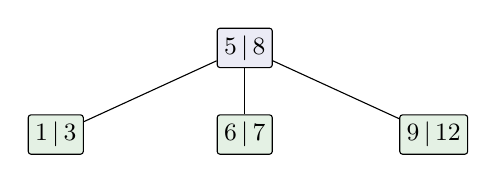
\begin{tikzpicture}[bt, level 1/.style={sibling distance=2.4cm}]
\node {5\sep 8}
  child {node[leaf] {1\sep 3}}
  child {node[leaf] {6\sep 7}}
  child {node[leaf] {9\sep 12}};
\end{tikzpicture}\\
{\scriptsize Final B-tree: 2 levels; every key appears once and carries its own data pointer.}
\end{exbox}

\subsection{B-tree deletion (summary)}
\begin{itemize}
  \item \textbf{Key in a leaf}, leaf stays at least half full $\Rightarrow$ just remove it.
  \item \textbf{Key in an internal node} $\Rightarrow$ replace it with its \textbf{in-order predecessor or successor} (always in a leaf), then delete that from the leaf.
  \item \textbf{Underflow} (fewer than $\lceil p/2\rceil - 1$ keys) $\Rightarrow$ \textbf{borrow} from a sibling through the parent (rotation), or \textbf{merge} with a sibling \emph{plus the separating key pulled down from the parent}. This may propagate upward, and if the root becomes empty, height $-1$.
\end{itemize}

\subsection{B-tree index slides (as given in the course)}
\begin{itemize}
  \item B-tree index is the widely used data structure for \textbf{tree-based indexing}. It is a \textbf{balanced multilevel} search tree.
  \item All leaf nodes hold actual data pointers, and the leaves are interlinked by a linked list, supporting \textbf{random and sequential access}. (Strictly, linked leaves are a B$^+$-tree feature.)
  \item \textbf{Internal nodes:} at least $\lceil n/2 \rceil$ pointers (except the root), at most $n$ pointers.
  \item \textbf{Leaf nodes:} at least $\lceil n/2 \rceil$ record pointers and keys; at most $n$. Every leaf has one block pointer $P$ to the next leaf.
\end{itemize}

%=====================================================================
\section{B$^+$-Tree}

\subsection{Properties}
\begin{itemize}
  \item A \textbf{balanced multiway} search tree used as a dynamic multilevel index. The slides say ``balanced binary search tree''; it is really $m$-ary.
  \item \textbf{All leaves at the same height}: every root-to-leaf path has the same length.
  \item \textbf{Internal nodes hold only keys + child pointers.} They are just ``signposts'' (a sparse index over the leaves).
  \item \textbf{Leaves hold every key}, each with a pointer to its record (or bucket of records).
  \item \textbf{Leaves are linked} in key order (next-leaf pointer), which supports \textbf{random} access (root$\to$leaf) and \textbf{sequential/range} access (leaf$\to$leaf).
\end{itemize}

\subsection{Node structure}
\[
\boxed{P_1 \mid K_1 \mid P_2 \mid K_2 \mid \cdots \mid P_{n-1} \mid K_{n-1} \mid P_n}
\qquad K_1 < K_2 < \dots < K_{n-1}
\]
\begin{itemize}
  \item \textbf{Internal node:} $P_i$ points to the subtree containing keys $x$ with $K_{i-1} \le x < K_i$.
  \item \textbf{Leaf node:} $P_i$ ($i = 1\dots n-1$) points to the record with key $K_i$; $P_n$ points to the \textbf{next leaf}.
  \item If $L_i, L_j$ are leaves with $i<j$, every key of $L_i$ is $\le$ every key of $L_j$.
\end{itemize}

\begin{exbox}[B$^+$-tree examples from the slides]
\centering
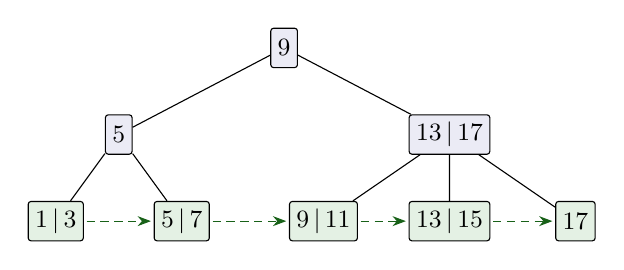
\begin{tikzpicture}[bt, level 1/.style={sibling distance=4.2cm}, level 2/.style={sibling distance=1.6cm}]
\node {9}
  child {node {5}
    child {node[leaf] (a1) {1\sep 3}}
    child {node[leaf] (a2) {5\sep 7}}}
  child {node {13\sep 17}
    child {node[leaf] (a3) {9\sep 11}}
    child {node[leaf] (a4) {13\sep 15}}
    child {node[leaf] (a5) {17}}};
\draw[link] (a1) -- (a2); \draw[link] (a2) -- (a3); \draw[link] (a3) -- (a4); \draw[link] (a4) -- (a5);
\end{tikzpicture}

\vspace{4pt}
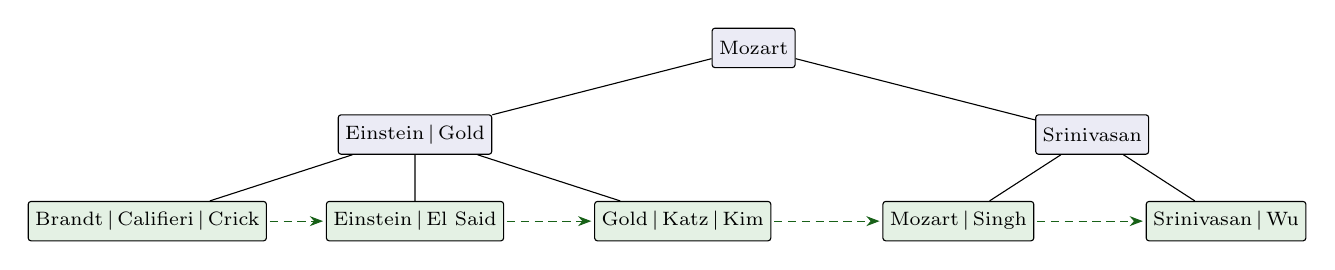
\begin{tikzpicture}[bt, level 1/.style={sibling distance=8.6cm}, level 2/.style={sibling distance=3.4cm}, every node/.append style={font=\scriptsize}]
\node {Mozart}
  child {node {Einstein\sep Gold}
    child {node[leaf] (b1) {Brandt\sep Califieri\sep Crick}}
    child {node[leaf] (b2) {Einstein\sep El Said}}
    child {node[leaf] (b3) {Gold\sep Katz\sep Kim}}}
  child {node {Srinivasan}
    child {node[leaf] (b4) {Mozart\sep Singh}}
    child {node[leaf] (b5) {Srinivasan\sep Wu}}};
\draw[link] (b1) -- (b2); \draw[link] (b2) -- (b3); \draw[link] (b3) -- (b4); \draw[link] (b4) -- (b5);
\end{tikzpicture}\\
{\scriptsize B$^+$-tree on \texttt{instructor.name}; each leaf key points to its instructor record (e.g.\ Brandt $\to$ 83821, Comp.\ Sci., 92000).}
\end{exbox}

\subsection{Order and occupancy rules}
\textbf{Order $m$} = maximum number of \textbf{child pointers} in a node. The slides give:

\begin{center}
\begin{tabular}{@{}lccc@{}}
\toprule
\textbf{Property} & \textbf{Root} & \textbf{Internal (non-root)} & \textbf{Leaf}\\\midrule
Maximum children & $m$ & $m$ & --\\
Minimum children & 2 (if internal) or 1 (if leaf) & $\lceil m/2 \rceil$ & --\\
Maximum keys & $m-1$ & $m-1$ & $m$ \textcolor{BrickRed}{(see note)}\\
Minimum keys & 1 (if internal) or 0 (if leaf) & $\lceil m/2 \rceil - 1$ & $\lceil m/2 \rceil$ \textcolor{BrickRed}{(see note)}\\
\bottomrule
\end{tabular}
\end{center}

\begin{warnbox}[Convention used in ALL worked examples (use this in the exam and state it)]
\begin{gather*}
\text{max keys (every node)} = m-1, \qquad
\text{min children (internal)} = \left\lceil \tfrac{m}{2} \right\rceil,\\
\text{min keys (internal)} = \left\lceil \tfrac{m}{2} \right\rceil - 1, \qquad
\text{min keys (leaf)} = \left\lceil \tfrac{m-1}{2} \right\rceil
\end{gather*}
The slide table says leaf max $= m$, but every slide example overflows a leaf at $m$ keys (order 3 at 3 keys, order 4 at 4 keys). So in practice leaf max $= m-1$. The construction-problem slide itself states leaf min $=\lceil (m-1)/2 \rceil$.
\end{warnbox}

\begin{center}
\begin{tabular}{@{}lcc@{}}
\toprule
 & $m=3$ & $m=4$\\\midrule
Max children & 3 & 4\\
Max keys (every node) & 2 & 3\\
Min children (non-root internal) & 2 & 2\\
Min keys (non-root internal) & 1 & 1\\
Min keys (leaf) & 1 & 2\\
Root & $\ge 2$ children (unless it is a leaf) & same\\
\bottomrule
\end{tabular}
\end{center}

\subsection{Search}
\begin{enumerate}
  \item Start at the root. In each internal node, follow the pointer to the left of the first key $> x$ (or the last pointer if $x \ge$ every key).
  \item At the leaf, look for $x$.
  \item \textbf{Range query $[a,b]$}: find the leaf for $a$, then follow the leaf links until a key $> b$.
\end{enumerate}
\[
\text{Cost} = \text{height} \approx \left\lceil \log_{\lceil m/2 \rceil} N \right\rceil \text{ (worst case)}, \qquad (+1 \text{ to read the data block})
\]
E.g.\ $N=10^6$, $m=100$: $\lceil \log_{50} 10^6 \rceil = \lceil 3.53 \rceil = 4$ levels (usually 3), against $\approx 17$ for binary search on a sorted file of 100,000 blocks.

%=====================================================================
\section{B$^+$-Tree Insertion}

\begin{keybox}[Algorithm]
\begin{enumerate}
  \item Every key is inserted into a \textbf{leaf}: search for the correct leaf $N$.
  \item Insert the key in sorted order.
    \begin{itemize}
      \item \textbf{Case I} -- leaf not full $\Rightarrow$ done.
      \item \textbf{Case II} -- leaf full $\Rightarrow$ \textbf{overflow}. Transfer a key to a sibling with room, \textbf{or split}:
    \end{itemize}
  \item \textbf{Leaf split:} left leaf keeps $\lfloor m/2 \rfloor$ keys, the right gets the rest. \textbf{Copy} the first key of the right leaf \textbf{up} into the parent; it also stays in the leaf.
  \item \textbf{Internal split:} the middle key \textbf{moves up} (push up, not kept in either half).
  \item If the parent overflows, repeat. If the \textbf{root splits}, a new root is created and \textbf{height $+1$}.
\end{enumerate}
\textbf{Leaf split $\to$ COPY up.\quad Internal split $\to$ PUSH up.}
\end{keybox}

%---------------------------------------------------------------
\begin{exbox}[Example 1 (slides): order $m=3$, insert 5, 15, 25, 35, 45]
\small
Max keys 2, min internal keys 1, leaf capacity 2.
\begin{itemize}
  \item Insert 5, 15: [5 15].
  \item Insert 25: [5 15 25] overflow $\to$ [5] $\mid$ [15 25], \textbf{copy 15} up.
  \item Insert 35: leaf [15 25 35] overflow $\to$ [15] $\mid$ [25 35], copy 25 up $\to$ root [15 25].
  \item Insert 45: leaf [25 35 45] overflow $\to$ [25] $\mid$ [35 45], copy 35 up $\to$ root [15 25 35] overflow $\to$ \textbf{internal split, push 25 up} $\to$ new root.
\end{itemize}
\centering
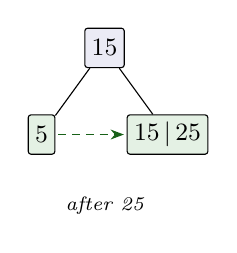
\begin{tikzpicture}[bt, level 1/.style={sibling distance=1.6cm}]
\node {15} child {node[leaf] (x1) {5}} child {node[leaf] (x2) {15\sep 25}};
\draw[link] (x1) -- (x2);
\node[tcap] at (0,-2) {after 25};
\end{tikzpicture}\hspace{8mm}
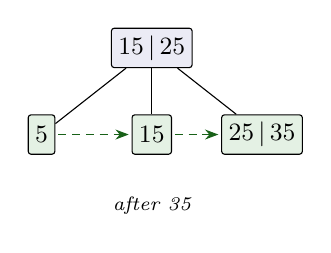
\begin{tikzpicture}[bt, level 1/.style={sibling distance=1.4cm}]
\node {15\sep 25} child {node[leaf] (y1) {5}} child {node[leaf] (y2) {15}} child {node[leaf] (y3) {25\sep 35}};
\draw[link] (y1) -- (y2); \draw[link] (y2) -- (y3);
\node[tcap] at (0,-2) {after 35};
\end{tikzpicture}\hspace{8mm}
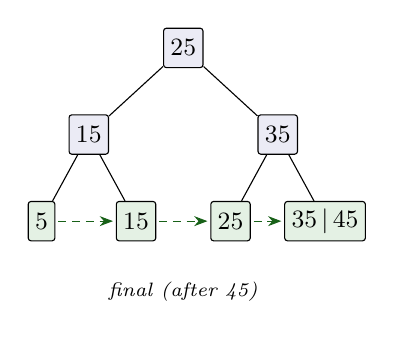
\begin{tikzpicture}[bt, level 1/.style={sibling distance=2.4cm}, level 2/.style={sibling distance=1.2cm}]
\node {25}
  child {node {15} child {node[leaf] (z1) {5}} child {node[leaf] (z2) {15}}}
  child {node {35} child {node[leaf] (z3) {25}} child {node[leaf] (z4) {35\sep 45}}};
\draw[link] (z1) -- (z2); \draw[link] (z2) -- (z3); \draw[link] (z3) -- (z4);
\node[tcap] at (0,-3.1) {final (after 45)};
\end{tikzpicture}
\end{exbox}

%---------------------------------------------------------------
\begin{exbox}[Example 2 (slides): order $m=4$, insert 10, 4, 90, 8, 1]
\small
Max keys 3. \; Insert 10, 4, 90 $\to$ [4 10 90] (full). \; Insert 8 $\to$ [4 8 10 90] overflow $\to$ split [4 8] $\mid$ [10 90], copy 10 up. \; Insert 1 $\to$ $1<10$ $\to$ left leaf [1 4 8] (fits).

\centering
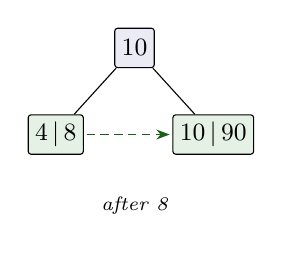
\begin{tikzpicture}[bt, level 1/.style={sibling distance=2cm}]
\node {10} child {node[leaf] (p1) {4\sep 8}} child {node[leaf] (p2) {10\sep 90}};
\draw[link] (p1) -- (p2);
\node[tcap] at (0,-2) {after 8};
\end{tikzpicture}\hspace{12mm}
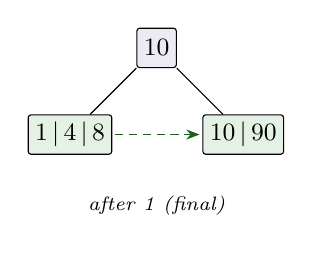
\begin{tikzpicture}[bt, level 1/.style={sibling distance=2.2cm}]
\node {10} child {node[leaf] (q1) {1\sep 4\sep 8}} child {node[leaf] (q2) {10\sep 90}};
\draw[link] (q1) -- (q2);
\node[tcap] at (0,-2) {after 1 (final)};
\end{tikzpicture}
\end{exbox}

%---------------------------------------------------------------
\begin{exbox}[Example 3 (slide problem): order $m=4$, insert 2, 4, 6, 8, 10, 12, 14, 16, 18, 20]
\small
Max keys 3, min internal keys 1, min leaf keys 2; promote the first key of the right node.
\begin{itemize}
  \item 2, 4, 6 $\to$ [2 4 6]. \; 8 $\to$ [2 4 6 8] overflow $\to$ [2 4] $\mid$ [6 8], promote 6.
  \item 10 $\to$ [6 8 10]. \; 12 $\to$ overflow $\to$ [6 8] $\mid$ [10 12], promote 10 $\to$ root [6 10].
  \item 14 $\to$ [10 12 14]. \; 16 $\to$ overflow $\to$ [10 12] $\mid$ [14 16], promote 14 $\to$ root [6 10 14].
  \item 18 $\to$ [14 16 18]. \; 20 $\to$ overflow $\to$ [14 16] $\mid$ [18 20], promote 18 $\to$ root [6 10 14 18] \textbf{overflow} (max 3).
  \item \textbf{Root split:} left [6 10], \textbf{push 14 up}, right [18] $\Rightarrow$ height increases.
\end{itemize}
\centering
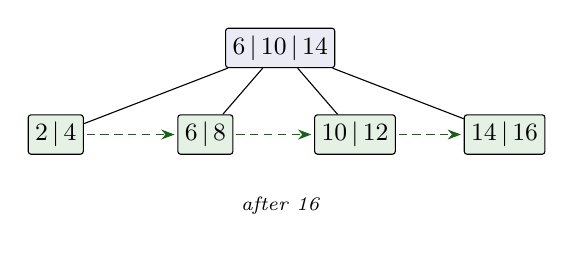
\begin{tikzpicture}[bt, level 1/.style={sibling distance=1.9cm}]
\node {6\sep 10\sep 14}
  child {node[leaf] (r1) {2\sep 4}} child {node[leaf] (r2) {6\sep 8}}
  child {node[leaf] (r3) {10\sep 12}} child {node[leaf] (r4) {14\sep 16}};
\draw[link] (r1) -- (r2); \draw[link] (r2) -- (r3); \draw[link] (r3) -- (r4);
\node[tcap] at (0,-2) {after 16};
\end{tikzpicture}\\[4pt]
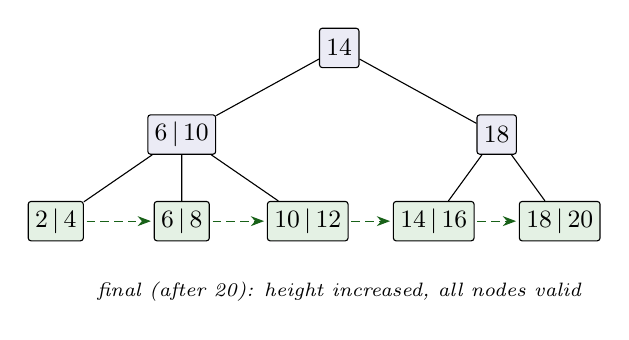
\begin{tikzpicture}[bt, level 1/.style={sibling distance=4cm}, level 2/.style={sibling distance=1.6cm}]
\node {14}
  child {node {6\sep 10}
    child {node[leaf] (s1) {2\sep 4}} child {node[leaf] (s2) {6\sep 8}} child {node[leaf] (s3) {10\sep 12}}}
  child {node {18}
    child {node[leaf] (s4) {14\sep 16}} child {node[leaf] (s5) {18\sep 20}}};
\draw[link] (s1) -- (s2); \draw[link] (s2) -- (s3); \draw[link] (s3) -- (s4); \draw[link] (s4) -- (s5);
\node[tcap] at (0,-3.1) {final (after 20): height increased, all nodes valid};
\end{tikzpicture}
\end{exbox}

%---------------------------------------------------------------
\begin{exbox}[Example 4 (slide homework): keys F, S, Q, K, C, L, H, T, V, W, M, R]
\small
\textbf{Order 3} (max 2 keys; leaf split 1 $\mid$ 2 with copy-up; internal split pushes the middle up):\\
F $\to$ [F]; S $\to$ [F S]; Q $\to$ [F Q S] split $\to$ [F] $\mid$ [Q S], root [Q];
K $\to$ [F K]; C $\to$ [C F K] split $\to$ [C] $\mid$ [F K], root [F Q];
L $\to$ [F K L] split $\to$ [F] $\mid$ [K L], root [F K Q] overflow $\to$ push K: root [K], internals [F], [Q];
H $\to$ [F H]; T $\to$ [Q S T] split $\to$ [Q] $\mid$ [S T], internal [Q S];
V $\to$ [S T V] split $\to$ [S] $\mid$ [T V], internal [Q S T] overflow $\to$ push S: root [K S], internals [Q], [T];
W $\to$ [T V W] split $\to$ [T] $\mid$ [V W], internal [T V];
M $\to$ [K L M] split $\to$ [K] $\mid$ [L M], internal [L Q];
R $\to$ [Q R].

\centering
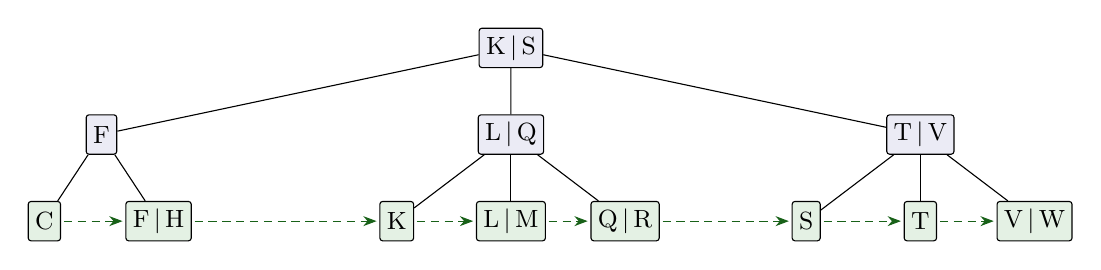
\begin{tikzpicture}[bt, level 1/.style={sibling distance=5.2cm}, level 2/.style={sibling distance=1.45cm}]
\node {K\sep S}
  child {node {F}
    child {node[leaf] (h1) {C}} child {node[leaf] (h2) {F\sep H}}}
  child {node {L\sep Q}
    child {node[leaf] (h3) {K}} child {node[leaf] (h4) {L\sep M}} child {node[leaf] (h5) {Q\sep R}}}
  child {node {T\sep V}
    child {node[leaf] (h6) {S}} child {node[leaf] (h7) {T}} child {node[leaf] (h8) {V\sep W}}};
\draw[link] (h1) -- (h2); \draw[link] (h2) -- (h3); \draw[link] (h3) -- (h4); \draw[link] (h4) -- (h5);
\draw[link] (h5) -- (h6); \draw[link] (h6) -- (h7); \draw[link] (h7) -- (h8);
\end{tikzpicture}

\raggedright
\textbf{Order 4} (max 3 keys; leaf split 2 $\mid$ 2 with copy-up):\\
F, S, Q $\to$ [F Q S]; K $\to$ [F K Q S] split $\to$ [F K] $\mid$ [Q S], root [Q];
C $\to$ [C F K]; L $\to$ [C F K L] split $\to$ [C F] $\mid$ [K L], root [K Q];
H $\to$ [C F H]; T $\to$ [Q S T]; V $\to$ [Q S T V] split $\to$ [Q S] $\mid$ [T V], root [K Q T];
W $\to$ [T V W]; M $\to$ [K L M]; R $\to$ [Q R S].

\centering
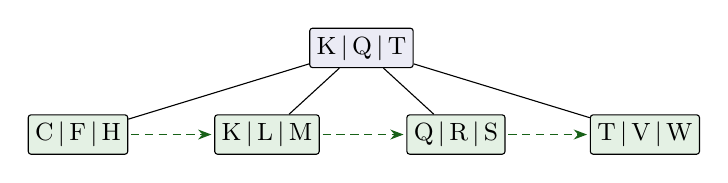
\begin{tikzpicture}[bt, level 1/.style={sibling distance=2.4cm}]
\node {K\sep Q\sep T}
  child {node[leaf] (g1) {C\sep F\sep H}} child {node[leaf] (g2) {K\sep L\sep M}}
  child {node[leaf] (g3) {Q\sep R\sep S}} child {node[leaf] (g4) {T\sep V\sep W}};
\draw[link] (g1) -- (g2); \draw[link] (g2) -- (g3); \draw[link] (g3) -- (g4);
\end{tikzpicture}
\end{exbox}

%---------------------------------------------------------------
\begin{exbox}[Example 5 (textbook keys): B$^+$-tree of order 3, insert 8, 5, 1, 7, 3, 12, 9, 6]
\small
8, 5 $\to$ [5 8]; \;1 $\to$ [1] $\mid$ [5 8], root [5]; \;7 $\to$ [5 7 8] split $\to$ [5] $\mid$ [7 8], root [5 7]; \;3 $\to$ [1 3];\;
12 $\to$ [7 8 12] split $\to$ [7] $\mid$ [8 12], copy 8 $\to$ root [5 7 8] overflow $\to$ push 7;\;
9 $\to$ [8 9 12] split $\to$ [8] $\mid$ [9 12], copy 9 $\to$ internal [8 9]; \;6 $\to$ [5 6].

\centering
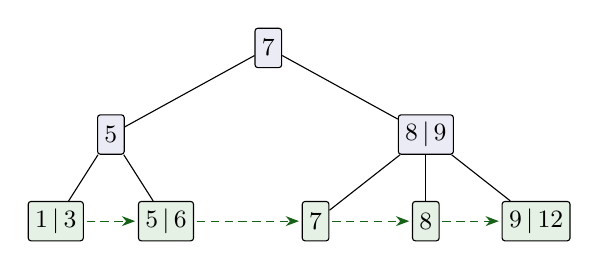
\begin{tikzpicture}[bt, level 1/.style={sibling distance=4cm}, level 2/.style={sibling distance=1.4cm}]
\node {7}
  child {node {5} child {node[leaf] (e1) {1\sep 3}} child {node[leaf] (e2) {5\sep 6}}}
  child {node {8\sep 9} child {node[leaf] (e3) {7}} child {node[leaf] (e4) {8}} child {node[leaf] (e5) {9\sep 12}}};
\draw[link] (e1) -- (e2); \draw[link] (e2) -- (e3); \draw[link] (e3) -- (e4); \draw[link] (e4) -- (e5);
\end{tikzpicture}\\
{\scriptsize Compare with the B-tree of the same keys (\S2.2): the B-tree has 2 levels with each key once; the B$^+$-tree has 3 levels, and keys 5, 7, 8, 9 appear twice.}
\end{exbox}

%=====================================================================
\section{B$^+$-Tree Deletion}

\begin{keybox}[Algorithm]
\begin{enumerate}
  \item Find the leaf $N$ containing $K$ and delete $K$.
  \item If $N$ still has \textbf{at least the minimum} keys $\Rightarrow$ done. Update a parent separator if needed.
  \item Otherwise \textbf{underflow}:
    \begin{itemize}
      \item \textbf{Borrow (redistribute)} a key from an immediate sibling that has more than the minimum, and update the parent separator; \textbf{or}
      \item \textbf{Merge} $N$ with a sibling and remove the separator from the parent. The parent may underflow in turn, so repeat upward.
    \end{itemize}
  \item If the root ends up with no keys (one child), remove it: \textbf{height $-1$}.
\end{enumerate}
\end{keybox}

\subsection{Deletion cases (slides, order $m=3$: max 2 keys, min 1 key per non-root node)}

\begin{center}
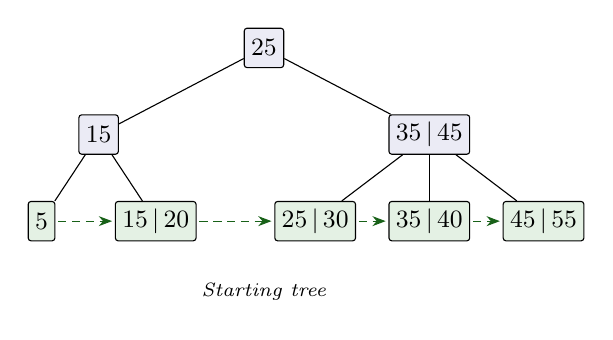
\begin{tikzpicture}[bt, level 1/.style={sibling distance=4.2cm}, level 2/.style={sibling distance=1.45cm}]
\node {25}
  child {node {15} child {node[leaf] (d1) {5}} child {node[leaf] (d2) {15\sep 20}}}
  child {node {35\sep 45} child {node[leaf] (d3) {25\sep 30}} child {node[leaf] (d4) {35\sep 40}} child {node[leaf] (d5) {45\sep 55}}};
\draw[link] (d1) -- (d2); \draw[link] (d2) -- (d3); \draw[link] (d3) -- (d4); \draw[link] (d4) -- (d5);
\node[tcap] at (0,-3.1) {Starting tree};
\end{tikzpicture}
\end{center}

\newcommand{\delcase}[4]{%
\begin{minipage}[t]{0.49\linewidth}
\textbf{#1}\\ {\small #2}\\[2pt]
\centering #3\\ {\scriptsize #4}
\end{minipage}}

\delcase{Case I(a) -- Delete 40}{Key only in a leaf that has more than the minimum $\Rightarrow$ simply delete.}{%
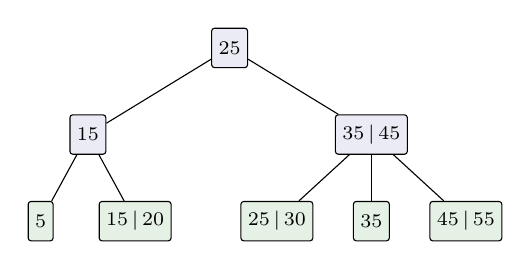
\begin{tikzpicture}[bt, level 1/.style={sibling distance=3.6cm}, level 2/.style={sibling distance=1.2cm}, every node/.append style={font=\scriptsize}]
\node {25}
  child {node {15} child {node[leaf] {5}} child {node[leaf] {15\sep 20}}}
  child {node {35\sep 45} child {node[leaf] {25\sep 30}} child {node[leaf] {35}} child {node[leaf] {45\sep 55}}};
\end{tikzpicture}}{Leaf [35 40] $\to$ [35].}\hfill
\delcase{Case I(b) -- Delete 5}{Leaf at the minimum $\Rightarrow$ delete, borrow from the immediate sibling, update the parent.}{%
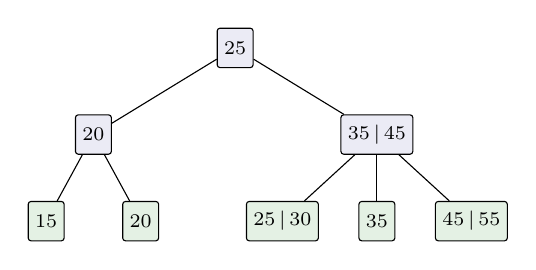
\begin{tikzpicture}[bt, level 1/.style={sibling distance=3.6cm}, level 2/.style={sibling distance=1.2cm}, every node/.append style={font=\scriptsize}]
\node {25}
  child {node {20} child {node[leaf] {15}} child {node[leaf] {20}}}
  child {node {35\sep 45} child {node[leaf] {25\sep 30}} child {node[leaf] {35}} child {node[leaf] {45\sep 55}}};
\end{tikzpicture}}{Borrow 15 from [15 20]; parent 15 $\to$ 20.}

\vspace{6pt}
\delcase{Case II(a) -- Delete 45}{Key in both a leaf and an internal node $\Rightarrow$ delete from the leaf, replace the internal key with its in-order successor.}{%
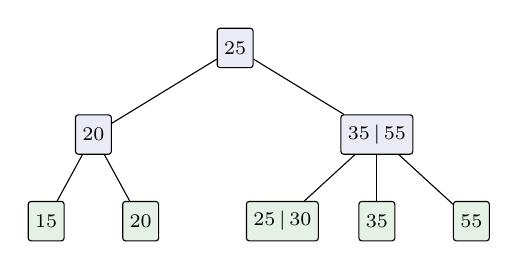
\begin{tikzpicture}[bt, level 1/.style={sibling distance=3.6cm}, level 2/.style={sibling distance=1.2cm}, every node/.append style={font=\scriptsize}]
\node {25}
  child {node {20} child {node[leaf] {15}} child {node[leaf] {20}}}
  child {node {35\sep 55} child {node[leaf] {25\sep 30}} child {node[leaf] {35}} child {node[leaf] {55}}};
\end{tikzpicture}}{Leaf [45 55] $\to$ [55]; internal [35 45] $\to$ [35 55].}\hfill
\delcase{Case II(b) -- Delete 35}{Leaf drops below the minimum $\Rightarrow$ borrow from the sibling through the parent; the borrowed key fills the internal node.}{%
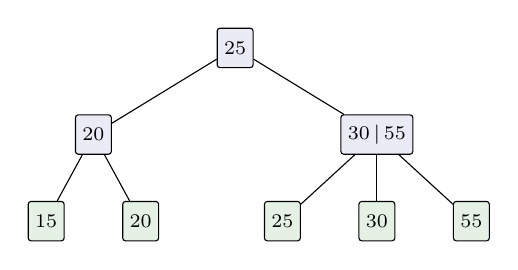
\begin{tikzpicture}[bt, level 1/.style={sibling distance=3.6cm}, level 2/.style={sibling distance=1.2cm}, every node/.append style={font=\scriptsize}]
\node {25}
  child {node {20} child {node[leaf] {15}} child {node[leaf] {20}}}
  child {node {30\sep 55} child {node[leaf] {25}} child {node[leaf] {30}} child {node[leaf] {55}}};
\end{tikzpicture}}{Borrow 30 from [25 30]; internal [35 55] $\to$ [30 55].}

\vspace{6pt}
\delcase{Case II(c) -- Delete 25}{Underflow reaches the parent $\Rightarrow$ merge with the sibling, update the grandparent with the in-order successor.}{%
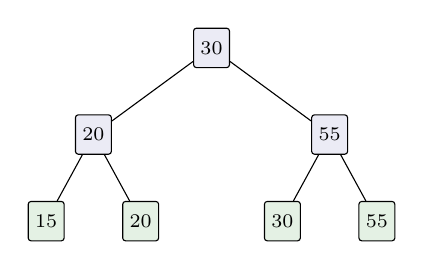
\begin{tikzpicture}[bt, level 1/.style={sibling distance=3cm}, level 2/.style={sibling distance=1.2cm}, every node/.append style={font=\scriptsize}]
\node {30}
  child {node {20} child {node[leaf] {15}} child {node[leaf] {20}}}
  child {node {55} child {node[leaf] {30}} child {node[leaf] {55}}};
\end{tikzpicture}}{Empty leaf merges away; root 25 $\to$ 30; internal [30 55] $\to$ [55].}\hfill
\delcase{Case III -- Delete 55}{Underflow propagates to the root $\Rightarrow$ root becomes empty and is removed; \textbf{height $-1$}.}{%
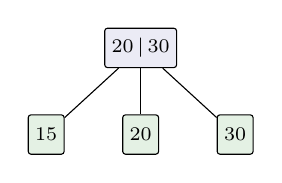
\begin{tikzpicture}[bt, level 1/.style={sibling distance=1.2cm}, every node/.append style={font=\scriptsize}]
\node {20\sep 30}
  child {node[leaf] {15}} child {node[leaf] {20}} child {node[leaf] {30}};
\end{tikzpicture}}{Internal [55] underflows, sibling [20] can't lend $\Rightarrow$ root 30 comes down: [20 30].}

\subsection{Deletion example from the construction problem (order $m=4$; delete 6, 8, 10, 12)}
\begin{exbox}[Start: final tree of Example 3 (min leaf keys 2, min internal keys 1)]
\small
\begin{enumerate}
  \item \textbf{Delete 6:} [6 8] $\to$ [8] underflow. The siblings [2 4] and [10 12] have exactly 2 keys (can't lend) $\Rightarrow$ \textbf{merge left}: [2 4 8]. Remove separator 6 $\to$ parent [10].
  \item \textbf{Delete 8:} [2 4 8] $\to$ [2 4], still valid.
  \item \textbf{Delete 10:} [10 12] $\to$ [12] underflow. Left sibling [2 4] has only 2 $\Rightarrow$ merge: [2 4 12]. Parent [10] now has 0 keys $\Rightarrow$ \textbf{internal underflow}.
  \item \textbf{Internal merge:} merge with sibling [18], \textbf{bringing down root key 14} $\Rightarrow$ [14 18]. Root empty $\Rightarrow$ removed, \textbf{height reduced}.
  \item \textbf{Delete 12} (not shown on the slides): [2 4 12] $\to$ [2 4], still valid.
\end{enumerate}
\centering
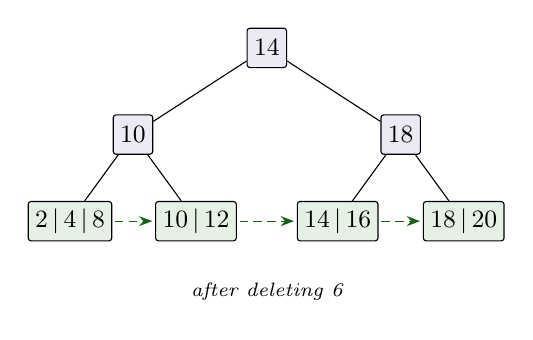
\begin{tikzpicture}[bt, level 1/.style={sibling distance=3.4cm}, level 2/.style={sibling distance=1.6cm}]
\node {14}
  child {node {10} child {node[leaf] (t1) {2\sep 4\sep 8}} child {node[leaf] (t2) {10\sep 12}}}
  child {node {18} child {node[leaf] (t3) {14\sep 16}} child {node[leaf] (t4) {18\sep 20}}};
\draw[link] (t1) -- (t2); \draw[link] (t2) -- (t3); \draw[link] (t3) -- (t4);
\node[tcap] at (0,-3.1) {after deleting 6};
\end{tikzpicture}\hspace{6mm}
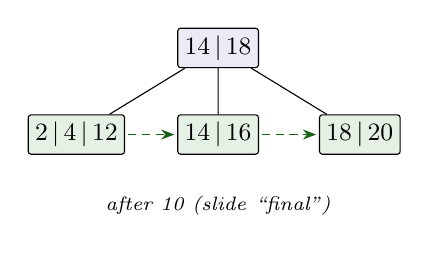
\begin{tikzpicture}[bt, level 1/.style={sibling distance=1.8cm}]
\node {14\sep 18}
  child {node[leaf] (u1) {2\sep 4\sep 12}} child {node[leaf] (u2) {14\sep 16}} child {node[leaf] (u3) {18\sep 20}};
\draw[link] (u1) -- (u2); \draw[link] (u2) -- (u3);
\node[tcap] at (0,-2) {after 10 (slide ``final'')};
\end{tikzpicture}\hspace{6mm}
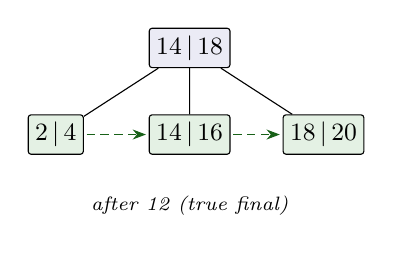
\begin{tikzpicture}[bt, level 1/.style={sibling distance=1.7cm}]
\node {14\sep 18}
  child {node[leaf] (v1) {2\sep 4}} child {node[leaf] (v2) {14\sep 16}} child {node[leaf] (v3) {18\sep 20}};
\draw[link] (v1) -- (v2); \draw[link] (v2) -- (v3);
\node[tcap] at (0,-2) {after 12 (true final)};
\end{tikzpicture}
\end{exbox}

\subsection{Delete 52 (slide -- result not shown there)}
\begin{exbox}[Solution with leaf min = 2]
\small
Leaf [41 52] $\to$ [41] underflows. The right sibling [58 59 61] has 3 keys $>$ min $\Rightarrow$ \textbf{borrow 58} $\Rightarrow$ leaves [41 58] and [59 61]; parent separator 58 $\to$ \textbf{59}.

\centering
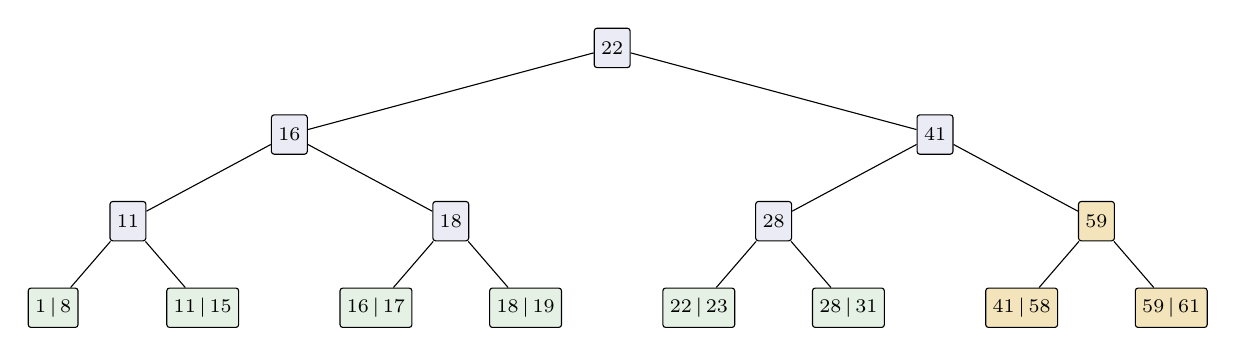
\begin{tikzpicture}[bt, level 1/.style={sibling distance=8.2cm}, level 2/.style={sibling distance=4.1cm}, level 3/.style={sibling distance=1.9cm}, every node/.append style={font=\scriptsize}]
\node {22}
  child {node {16}
    child {node {11} child {node[leaf] {1\sep 8}} child {node[leaf] {11\sep 15}}}
    child {node {18} child {node[leaf] {16\sep 17}} child {node[leaf] {18\sep 19}}}}
  child {node {41}
    child {node {28} child {node[leaf] {22\sep 23}} child {node[leaf] {28\sep 31}}}
    child {node[fill=Goldenrod!30] {59} child {node[leaf,fill=Goldenrod!30] {41\sep 58}} child {node[leaf,fill=Goldenrod!30] {59\sep 61}}}};
\end{tikzpicture}\\
{\scriptsize Before: the right-most internal node was [58] with leaves [41 52] and [58 59 61]. The highlighted nodes changed. (If the leaf minimum were 1, [41] would be valid and nothing else would change.)}
\end{exbox}

%=====================================================================
\section{B-Tree vs.\ B$^+$-Tree}

\begin{tabularx}{\linewidth}{@{}X X@{}}
\toprule
\textbf{B-tree} & \textbf{B$^+$-tree}\\\midrule
Data pointers in \textbf{all} nodes & Data pointers \textbf{only in the leaves}\\
Each key appears \textbf{once} & Internal keys are \textbf{repeated} in the leaves\\
No leaf chain & \textbf{Leaves linked} $\Rightarrow$ fast range/sequential scans\\
Internal nodes store $\langle K, Pr \rangle$ $\Rightarrow$ \textbf{lower fan-out} & Internal nodes store only keys + tree pointers $\Rightarrow$ \textbf{higher fan-out, shallower tree}\\
Search may stop early at an internal node & Search always ends at a leaf (uniform cost)\\
Split: median \textbf{moves} up & Leaf split: \textbf{copy} up; internal split: \textbf{move} up\\
Deletion from internal nodes is complex & Deletion always starts at a leaf\\
\bottomrule
\end{tabularx}

\subsection*{Capacity calculation (Elmasri example)}
Given: key $V=9$ B, block $B=512$ B, data pointer $Pr=7$ B, block pointer $P=6$ B; nodes about 69\% full.

\textbf{B-tree order:}
\[
p\,P + (p-1)(Pr+V) \le B \;\Rightarrow\; 6p + 16(p-1) \le 512 \;\Rightarrow\; 22p \le 528 \;\Rightarrow\; p = 24
\]
At 69\%: $\approx 16$ pointers, 15 keys per node.

\textbf{B$^+$-tree orders:}
\[
\text{internal: } p\,P + (p-1)V \le B \Rightarrow 15p \le 521 \Rightarrow p = 34; \qquad
\text{leaf: } p_{leaf}(Pr+V) + P \le B \Rightarrow 16\,p_{leaf} + 6 \le 512 \Rightarrow p_{leaf} = 31
\]
At 69\%: internal $\approx 23$ pointers (22 keys), leaf $\approx 21$ data pointers.

\begin{center}
\small
\begin{tabular}{@{}lrrr@{\hspace{1.2cm}}lrrr@{}}
\toprule
\multicolumn{4}{@{}c}{\textbf{B-tree}} & \multicolumn{4}{c@{}}{\textbf{B$^+$-tree}}\\
Level & Nodes & Keys & Pointers & Level & Nodes & Keys & Pointers\\\midrule
Root & 1 & 15 & 16 & Root & 1 & 22 & 23\\
Level 1 & 16 & 240 & 256 & Level 1 & 23 & 506 & 529\\
Level 2 & 256 & 3,840 & 4,096 & Level 2 & 529 & 11,638 & 12,167\\
Level 3 & 4,096 & 61,440 & -- & Leaves & 12,167 & -- & 255,507 data ptrs\\\midrule
\textbf{Total} & & \textbf{65,535} & & \textbf{Total} & & & \textbf{255,507}\\
\bottomrule
\end{tabular}
\end{center}
With the same 4 levels the B$^+$-tree indexes about \textbf{4$\times$ more records}, because its internal nodes don't waste space on data pointers. \textbf{This is why DBMSs use B$^+$-trees.}

%=====================================================================
\section{Index Definition in SQL}
\begin{verbatim}
CREATE INDEX <index-name> ON <relation-name> (<attribute-list>);
CREATE INDEX b_index ON branch(branch_name);
CREATE UNIQUE INDEX ...      -- also enforces that the search key is a candidate key
DROP INDEX <index-name>;
\end{verbatim}
Most RDBMSs build a B$^+$-tree by default (e.g.\ MySQL InnoDB's primary key is a clustered B$^+$-tree).

%=====================================================================
\section{Slide Errata}
\begin{tabularx}{\linewidth}{@{}l X@{}}
\toprule
\textbf{Slide} & \textbf{Issue $\to$ correction}\\\midrule
Main 136, 138; idx 38--39 & ``Balanced \emph{binary} search tree'' $\to$ balanced \textbf{multiway} tree. Linked leaves are a B$^+$-tree feature.\\
Main 138 & ``Lead nodes'' $\to$ leaf nodes; the ranges ``2--4 values, 3--5 children'' don't match $n=3$.\\
Main 147; idx 42, 49, 53 & Leaf max keys $=m$, leaf min $=\lceil m/2 \rceil$ $\to$ the examples use leaf max $m-1$ and leaf min $\lceil (m-1)/2 \rceil$.\\
Main 153--154 & ``Delete 52'' result not shown $\to$ see \S5.3.\\
Main 160 & ``Delete 6, 8, 10, 12'' -- 12 never deleted $\to$ final root [14 18] $\to$ [2 4], [14 16], [18 20].\\
\bottomrule
\end{tabularx}

%=====================================================================
\section{Quick Revision}
\begin{itemize}
  \item \textbf{B-tree:} data pointers in every node, each key once, median moves up on a split.
  \item \textbf{B$^+$-tree:} data pointers only in the leaves, leaves linked, higher fan-out $\Rightarrow$ shallower.
  \item Order $m$: max $m$ children, max $m-1$ keys; internal min $\lceil m/2 \rceil$ children ($\lceil m/2 \rceil-1$ keys); leaf min $\lceil (m-1)/2 \rceil$ keys; root $\ge 2$ children.
  \item Insert: always into a leaf. Overflow $\Rightarrow$ split; \textbf{leaf split copies up, internal split pushes up}. Root split $\Rightarrow$ height $+1$.
  \item Delete: always from a leaf. Underflow $\Rightarrow$ \textbf{borrow} from a sibling (update separator) else \textbf{merge} (remove separator). Empty root $\Rightarrow$ height $-1$.
  \item Internal key deleted $\Rightarrow$ replace it with the \textbf{in-order successor}.
  \item Search / insert / delete cost $\approx$ height $= O(\log_{\lceil m/2\rceil} N)$.
  \item Capacity formulas: B-tree $pP+(p-1)(Pr+V)\le B$; B$^+$ internal $pP+(p-1)V\le B$; B$^+$ leaf $p_{leaf}(Pr+V)+P\le B$.
\end{itemize}

\end{document}
